\documentclass{subfiles}

\begin{document}

\subsection{Stern-Gerlach-Experiment}
    Das \href{https://de.wikipedia.org/wiki/Stern-Gerlach-Versuch}{\emph{Stern-Gerlach Experiment}} weist die Richtungsquantelung des Drehimpulses nach. Dabei wird ein Strahl von Silberatomen durch ein inhomogenes Magnetfeld geschickt. Der schematische Aufbau des Experiments ist wiefolgt:
    \begin{figure}[H]
        \centering
        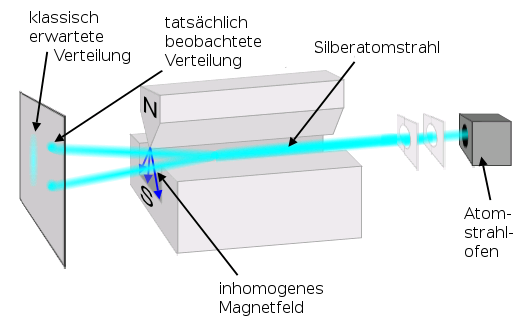
\includegraphics[width=7cm]{Bilddateien/SternGerlach.png}
        \caption{Schematischer Aufbau des Stern-Gerlach-Experiments.}
    \end{figure}
    Der Spinnachweis gelingt dabei dadurch, daß die Atome in zwei verschiedene Richtungen abgelenkt werden. 
    \begin{Aufgabe}
        \nr{} Zur Anschauung des Prizips betrachte das hinterlegte $\to$\href{https://en.wikipedia.org/wiki/File:Quantum_spin_and_the_Stern-Gerlach_experiment.ogv}{Video}.

        \nr{} Betrachte die hinterlegte $\to$\href{https://upload.wikimedia.org/wikipedia/commons/c/cb/Stern-Gerlach_Analyzer_Sequential_Series_E3.png}{Grafik} und erkläre die dazu führenden Prozesse. 
    \end{Aufgabe}
\end{document}